% Options for packages loaded elsewhere
% Options for packages loaded elsewhere
\PassOptionsToPackage{unicode}{hyperref}
\PassOptionsToPackage{hyphens}{url}
\PassOptionsToPackage{dvipsnames,svgnames,x11names}{xcolor}
%
\documentclass[
]{article}
\usepackage{xcolor}
\usepackage[top=0.75in,left=0.75in,bottom=0.75in,right=0.75in]{geometry}
\usepackage{amsmath,amssymb}
\setcounter{secnumdepth}{5}
\usepackage{iftex}
\ifPDFTeX
  \usepackage[T1]{fontenc}
  \usepackage[utf8]{inputenc}
  \usepackage{textcomp} % provide euro and other symbols
\else % if luatex or xetex
  \usepackage{unicode-math} % this also loads fontspec
  \defaultfontfeatures{Scale=MatchLowercase}
  \defaultfontfeatures[\rmfamily]{Ligatures=TeX,Scale=1}
\fi
\usepackage{lmodern}
\ifPDFTeX\else
  % xetex/luatex font selection
\fi
% Use upquote if available, for straight quotes in verbatim environments
\IfFileExists{upquote.sty}{\usepackage{upquote}}{}
\IfFileExists{microtype.sty}{% use microtype if available
  \usepackage[]{microtype}
  \UseMicrotypeSet[protrusion]{basicmath} % disable protrusion for tt fonts
}{}
\makeatletter
\@ifundefined{KOMAClassName}{% if non-KOMA class
  \IfFileExists{parskip.sty}{%
    \usepackage{parskip}
  }{% else
    \setlength{\parindent}{0pt}
    \setlength{\parskip}{6pt plus 2pt minus 1pt}}
}{% if KOMA class
  \KOMAoptions{parskip=half}}
\makeatother
% Make \paragraph and \subparagraph free-standing
\makeatletter
\ifx\paragraph\undefined\else
  \let\oldparagraph\paragraph
  \renewcommand{\paragraph}{
    \@ifstar
      \xxxParagraphStar
      \xxxParagraphNoStar
  }
  \newcommand{\xxxParagraphStar}[1]{\oldparagraph*{#1}\mbox{}}
  \newcommand{\xxxParagraphNoStar}[1]{\oldparagraph{#1}\mbox{}}
\fi
\ifx\subparagraph\undefined\else
  \let\oldsubparagraph\subparagraph
  \renewcommand{\subparagraph}{
    \@ifstar
      \xxxSubParagraphStar
      \xxxSubParagraphNoStar
  }
  \newcommand{\xxxSubParagraphStar}[1]{\oldsubparagraph*{#1}\mbox{}}
  \newcommand{\xxxSubParagraphNoStar}[1]{\oldsubparagraph{#1}\mbox{}}
\fi
\makeatother

\usepackage{color}
\usepackage{fancyvrb}
\newcommand{\VerbBar}{|}
\newcommand{\VERB}{\Verb[commandchars=\\\{\}]}
\DefineVerbatimEnvironment{Highlighting}{Verbatim}{commandchars=\\\{\}}
% Add ',fontsize=\small' for more characters per line
\usepackage{framed}
\definecolor{shadecolor}{RGB}{241,243,245}
\newenvironment{Shaded}{\begin{snugshade}}{\end{snugshade}}
\newcommand{\AlertTok}[1]{\textcolor[rgb]{0.68,0.00,0.00}{#1}}
\newcommand{\AnnotationTok}[1]{\textcolor[rgb]{0.37,0.37,0.37}{#1}}
\newcommand{\AttributeTok}[1]{\textcolor[rgb]{0.40,0.45,0.13}{#1}}
\newcommand{\BaseNTok}[1]{\textcolor[rgb]{0.68,0.00,0.00}{#1}}
\newcommand{\BuiltInTok}[1]{\textcolor[rgb]{0.00,0.23,0.31}{#1}}
\newcommand{\CharTok}[1]{\textcolor[rgb]{0.13,0.47,0.30}{#1}}
\newcommand{\CommentTok}[1]{\textcolor[rgb]{0.37,0.37,0.37}{#1}}
\newcommand{\CommentVarTok}[1]{\textcolor[rgb]{0.37,0.37,0.37}{\textit{#1}}}
\newcommand{\ConstantTok}[1]{\textcolor[rgb]{0.56,0.35,0.01}{#1}}
\newcommand{\ControlFlowTok}[1]{\textcolor[rgb]{0.00,0.23,0.31}{\textbf{#1}}}
\newcommand{\DataTypeTok}[1]{\textcolor[rgb]{0.68,0.00,0.00}{#1}}
\newcommand{\DecValTok}[1]{\textcolor[rgb]{0.68,0.00,0.00}{#1}}
\newcommand{\DocumentationTok}[1]{\textcolor[rgb]{0.37,0.37,0.37}{\textit{#1}}}
\newcommand{\ErrorTok}[1]{\textcolor[rgb]{0.68,0.00,0.00}{#1}}
\newcommand{\ExtensionTok}[1]{\textcolor[rgb]{0.00,0.23,0.31}{#1}}
\newcommand{\FloatTok}[1]{\textcolor[rgb]{0.68,0.00,0.00}{#1}}
\newcommand{\FunctionTok}[1]{\textcolor[rgb]{0.28,0.35,0.67}{#1}}
\newcommand{\ImportTok}[1]{\textcolor[rgb]{0.00,0.46,0.62}{#1}}
\newcommand{\InformationTok}[1]{\textcolor[rgb]{0.37,0.37,0.37}{#1}}
\newcommand{\KeywordTok}[1]{\textcolor[rgb]{0.00,0.23,0.31}{\textbf{#1}}}
\newcommand{\NormalTok}[1]{\textcolor[rgb]{0.00,0.23,0.31}{#1}}
\newcommand{\OperatorTok}[1]{\textcolor[rgb]{0.37,0.37,0.37}{#1}}
\newcommand{\OtherTok}[1]{\textcolor[rgb]{0.00,0.23,0.31}{#1}}
\newcommand{\PreprocessorTok}[1]{\textcolor[rgb]{0.68,0.00,0.00}{#1}}
\newcommand{\RegionMarkerTok}[1]{\textcolor[rgb]{0.00,0.23,0.31}{#1}}
\newcommand{\SpecialCharTok}[1]{\textcolor[rgb]{0.37,0.37,0.37}{#1}}
\newcommand{\SpecialStringTok}[1]{\textcolor[rgb]{0.13,0.47,0.30}{#1}}
\newcommand{\StringTok}[1]{\textcolor[rgb]{0.13,0.47,0.30}{#1}}
\newcommand{\VariableTok}[1]{\textcolor[rgb]{0.07,0.07,0.07}{#1}}
\newcommand{\VerbatimStringTok}[1]{\textcolor[rgb]{0.13,0.47,0.30}{#1}}
\newcommand{\WarningTok}[1]{\textcolor[rgb]{0.37,0.37,0.37}{\textit{#1}}}

\usepackage{longtable,booktabs,array}
\newcounter{none} % for unnumbered tables
\usepackage{calc} % for calculating minipage widths
% Correct order of tables after \paragraph or \subparagraph
\usepackage{etoolbox}
\makeatletter
\patchcmd\longtable{\par}{\if@noskipsec\mbox{}\fi\par}{}{}
\makeatother
% Allow footnotes in longtable head/foot
\IfFileExists{footnotehyper.sty}{\usepackage{footnotehyper}}{\usepackage{footnote}}
\makesavenoteenv{longtable}
\usepackage{graphicx}
\makeatletter
\newsavebox\pandoc@box
\newcommand*\pandocbounded[1]{% scales image to fit in text height/width
  \sbox\pandoc@box{#1}%
  \Gscale@div\@tempa{\textheight}{\dimexpr\ht\pandoc@box+\dp\pandoc@box\relax}%
  \Gscale@div\@tempb{\linewidth}{\wd\pandoc@box}%
  \ifdim\@tempb\p@<\@tempa\p@\let\@tempa\@tempb\fi% select the smaller of both
  \ifdim\@tempa\p@<\p@\scalebox{\@tempa}{\usebox\pandoc@box}%
  \else\usebox{\pandoc@box}%
  \fi%
}
% Set default figure placement to htbp
\def\fps@figure{htbp}
\makeatother





\setlength{\emergencystretch}{3em} % prevent overfull lines

\providecommand{\tightlist}{%
  \setlength{\itemsep}{0pt}\setlength{\parskip}{0pt}}



 


\makeatletter
\@ifpackageloaded{caption}{}{\usepackage{caption}}
\AtBeginDocument{%
\ifdefined\contentsname
  \renewcommand*\contentsname{Table of contents}
\else
  \newcommand\contentsname{Table of contents}
\fi
\ifdefined\listfigurename
  \renewcommand*\listfigurename{List of Figures}
\else
  \newcommand\listfigurename{List of Figures}
\fi
\ifdefined\listtablename
  \renewcommand*\listtablename{List of Tables}
\else
  \newcommand\listtablename{List of Tables}
\fi
\ifdefined\figurename
  \renewcommand*\figurename{Figure}
\else
  \newcommand\figurename{Figure}
\fi
\ifdefined\tablename
  \renewcommand*\tablename{Table}
\else
  \newcommand\tablename{Table}
\fi
}
\@ifpackageloaded{float}{}{\usepackage{float}}
\floatstyle{ruled}
\@ifundefined{c@chapter}{\newfloat{codelisting}{h}{lop}}{\newfloat{codelisting}{h}{lop}[chapter]}
\floatname{codelisting}{Listing}
\newcommand*\listoflistings{\listof{codelisting}{List of Listings}}
\makeatother
\makeatletter
\makeatother
\makeatletter
\@ifpackageloaded{caption}{}{\usepackage{caption}}
\@ifpackageloaded{subcaption}{}{\usepackage{subcaption}}
\makeatother
\usepackage{bookmark}
\IfFileExists{xurl.sty}{\usepackage{xurl}}{} % add URL line breaks if available
\urlstyle{same}
% fallback for those not using the hyperref driver hyperxmp:
\makeatletter
\@ifundefined{xmpquote}{\newcommand{\xmpquote}[1]{#1}}{}
\makeatother
\hypersetup{
  pdftitle={Lab Ten -- Point Estimation},
  colorlinks=true,
  linkcolor={blue},
  filecolor={Maroon},
  citecolor={Blue},
  urlcolor={Blue},
  pdfcreator={LaTeX via pandoc}}


\title{Lab Ten -- Point Estimation}
\author{}
\date{}
\begin{document}
\maketitle


\normalsize

\normalsize

\section{Lab 8 Notes}\label{lab-8-notes}

\subsection{Altham's Multiplicative Binomial
Distribution}\label{althams-multiplicative-binomial-distribution}

The PMF for Altham's Multiplicative Binomial Distribution is
\[f_X(x) = \frac{1}{c} {n \choose x} p^x (1-p)^{n-x} \theta^{x(n-x)}I(x \in \{0, 1, ..., n\})\]
where
\[c = \sum_{i=0}^n {n \choose i} p^i (1-p)^{n-i} \theta^{i(n-i)}.\] Just
so we start on the same page, I have included my \texttt{R} function for
computing probability using this distribution.

\normalsize

\begin{Shaded}
\begin{Highlighting}[numbers=left,,]
\NormalTok{daltbinom }\OtherTok{\textless{}{-}} \ControlFlowTok{function}\NormalTok{(x, size, prob, theta)\{}
\NormalTok{  normalizing.constant }\OtherTok{\textless{}{-}} \DecValTok{0}
  \ControlFlowTok{for}\NormalTok{(j }\ControlFlowTok{in} \DecValTok{0}\SpecialCharTok{:}\NormalTok{size)\{}
\NormalTok{    normalizing.constant }\OtherTok{\textless{}{-}}\NormalTok{ normalizing.constant }\SpecialCharTok{+} 
      \FunctionTok{choose}\NormalTok{(size, j) }\SpecialCharTok{*}\NormalTok{ prob}\SpecialCharTok{\^{}}\NormalTok{j }\SpecialCharTok{*}\NormalTok{ (}\DecValTok{1}\SpecialCharTok{{-}}\NormalTok{prob)}\SpecialCharTok{\^{}}\NormalTok{(size}\SpecialCharTok{{-}}\NormalTok{j) }\SpecialCharTok{*}\NormalTok{ theta}\SpecialCharTok{\^{}}\NormalTok{(j}\SpecialCharTok{*}\NormalTok{(size}\SpecialCharTok{{-}}\NormalTok{j))}
\NormalTok{  \}}
  \CommentTok{\# Probability Mass at x=x}
\NormalTok{  (}\DecValTok{1}\SpecialCharTok{/}\NormalTok{normalizing.constant) }\SpecialCharTok{*}
    \FunctionTok{choose}\NormalTok{(size, x) }\SpecialCharTok{*}\NormalTok{ prob}\SpecialCharTok{\^{}}\NormalTok{x }\SpecialCharTok{*}\NormalTok{ (}\DecValTok{1}\SpecialCharTok{{-}}\NormalTok{prob)}\SpecialCharTok{\^{}}\NormalTok{(size}\SpecialCharTok{{-}}\NormalTok{x) }\SpecialCharTok{*}\NormalTok{ theta}\SpecialCharTok{\^{}}\NormalTok{(x}\SpecialCharTok{*}\NormalTok{(size}\SpecialCharTok{{-}}\NormalTok{x)) }\SpecialCharTok{*}
\NormalTok{      (x}\SpecialCharTok{\textgreater{}=}\DecValTok{0}\NormalTok{)}\SpecialCharTok{*}\NormalTok{(x}\SpecialCharTok{\textless{}=}\NormalTok{size)}
\NormalTok{\}}
\end{Highlighting}
\end{Shaded}

\normalsize

\section{Altham's Multiplicative Beta Binomial
Distribution}\label{althams-multiplicative-beta-binomial-distribution}

The PMF for Altham's Multiplicative Beta Binomial Distribution is
\[f_X(x) = \left[\int_{0}^1 \left(\frac{1}{c} {n \choose x} p^x (1-p)^{n-x} \theta^{x(n-x)}\right)\left(\frac{\Gamma(\alpha+\beta)}{\Gamma(\alpha)\Gamma(\beta)} p^{\alpha-1}(1-p)^{\beta-1}\right) dp\right]I(x \in \{0, 1, ..., n\})\]

Prof.~Cipolli included \texttt{R} function for computing probability
using this distribution.

\normalsize

\begin{Shaded}
\begin{Highlighting}[numbers=left,,]
\NormalTok{daltbbinom.single }\OtherTok{\textless{}{-}} \ControlFlowTok{function}\NormalTok{(x, size, alpha, beta, theta)\{}
\NormalTok{    integrand }\OtherTok{\textless{}{-}} \ControlFlowTok{function}\NormalTok{(p) \{}
    \FunctionTok{sapply}\NormalTok{(p, }\CommentTok{\# integrate will pass in a vector, so we use sapply to apply the following}
           \ControlFlowTok{function}\NormalTok{(p\_val)\{}
             \CommentTok{\# f(x|p) * f(p|alpha, beta)}
             \FunctionTok{daltbinom}\NormalTok{(x, size, p\_val, theta) }\SpecialCharTok{*} \FunctionTok{dbeta}\NormalTok{(p\_val, alpha, beta)}
\NormalTok{           \}}
\NormalTok{    )}
\NormalTok{  \}}
  \CommentTok{\# Probability Mass at x=x}
  \CommentTok{\# integrate(integrand, lower = 0, upper = 1)$value * (x\textgreater{}=0)*(x\textless{}=size)}
  \CommentTok{\# I shrink the bounds below to avoid log(0)={-}infinty}
  \CommentTok{\# I use try() to catch when there is an error and avoid crashing}
\NormalTok{  res }\OtherTok{\textless{}{-}} \FunctionTok{try}\NormalTok{(}\FunctionTok{integrate}\NormalTok{(integrand, }\AttributeTok{lower =} \FloatTok{1e{-}7}\NormalTok{, }\AttributeTok{upper =} \DecValTok{1} \SpecialCharTok{{-}} \FloatTok{1e{-}7}\NormalTok{)}\SpecialCharTok{$}\NormalTok{value }\SpecialCharTok{*} 
\NormalTok{                  (x}\SpecialCharTok{\textgreater{}=}\DecValTok{0}\NormalTok{)}\SpecialCharTok{*}\NormalTok{(x}\SpecialCharTok{\textless{}=}\NormalTok{size), }
             \AttributeTok{silent =} \ConstantTok{TRUE}\NormalTok{)}
  \CommentTok{\# If there is an error, return a near{-}zero probability}
  \ControlFlowTok{if}\NormalTok{(}\FunctionTok{inherits}\NormalTok{(res, }\StringTok{"try{-}error"}\NormalTok{)) }\FunctionTok{return}\NormalTok{(}\FloatTok{0.1}\SpecialCharTok{\^{}}\DecValTok{6}\NormalTok{)}
  
\NormalTok{  res}
\NormalTok{\}}
\CommentTok{\# Write a function that works on a vector}
\NormalTok{daltbbinom }\OtherTok{\textless{}{-}} \ControlFlowTok{function}\NormalTok{(x, size, alpha, beta, theta)\{}
  \FunctionTok{sapply}\NormalTok{(}\AttributeTok{X=}\NormalTok{x, }\AttributeTok{FUN=}\NormalTok{daltbbinom.single, }\AttributeTok{size=}\NormalTok{size, }\AttributeTok{alpha=}\NormalTok{alpha, }\AttributeTok{beta=}\NormalTok{beta, }\AttributeTok{theta=}\NormalTok{theta)}
\NormalTok{\}}
\end{Highlighting}
\end{Shaded}

\normalsize

\section{Question 1}\label{question-1}

In Lab 8, we use Altham's Multiplicative Binomial Distribution. Your job
was to interpret the impact of \(\theta\) in that equation. In this lab,
we will model the number of legs won in a best of eleven (first to six)
match.

To help us think about the interpretation, something that was
challenging before, let's try something a little more manageable.

\subsection{Part a}\label{part-a}

Suppose a player has a 50\% chance of winning a specific leg, that is
let \(p=0.50\). Let's look at the probability they win (\(x=6\)) legs in
the match. Compute this probability over a sequence from \(\theta=0.5\)
to \(\theta=1.5\) and plot it using a line where the \(x\)-axis is
\(\theta\) and the \(y\)-axis is \(P(X=6)\).

\textbf{Solution}

\normalsize

\begin{Shaded}
\begin{Highlighting}[numbers=left,,]
\NormalTok{theta\_seq }\OtherTok{=} \FunctionTok{seq}\NormalTok{(}\FloatTok{0.5}\NormalTok{, }\FloatTok{1.5}\NormalTok{, }\AttributeTok{length.out=}\DecValTok{1000}\NormalTok{)}
\NormalTok{prob\_x6 }\OtherTok{=} \FunctionTok{rep}\NormalTok{(}\ConstantTok{NA}\NormalTok{, }\FunctionTok{length}\NormalTok{(theta\_seq))}
\ControlFlowTok{for}\NormalTok{(i }\ControlFlowTok{in} \DecValTok{1}\SpecialCharTok{:}\FunctionTok{length}\NormalTok{(theta\_seq))\{}
\NormalTok{  prob\_x6[i] }\OtherTok{=} \FunctionTok{daltbinom}\NormalTok{(}\AttributeTok{x=}\DecValTok{6}\NormalTok{, }\AttributeTok{size=}\DecValTok{11}\NormalTok{, }\AttributeTok{prob=}\FloatTok{0.50}\NormalTok{, }\AttributeTok{theta=}\NormalTok{theta\_seq[i])}
\NormalTok{\}}
\NormalTok{x6 }\OtherTok{\textless{}{-}} \FunctionTok{tibble}\NormalTok{(}\AttributeTok{theta =}\NormalTok{ theta\_seq,}
            \AttributeTok{prob  =}\NormalTok{ prob\_x6)}
\end{Highlighting}
\end{Shaded}

\normalsize

\scriptsize

\begin{Shaded}
\begin{Highlighting}[numbers=left,,]
\FunctionTok{ggplot}\NormalTok{(x6) }\SpecialCharTok{+}
  \FunctionTok{geom\_line}\NormalTok{(}\FunctionTok{aes}\NormalTok{(}\AttributeTok{x =}\NormalTok{ theta, }\AttributeTok{y =}\NormalTok{ prob), }\AttributeTok{color =} \StringTok{"darkorange3"}\NormalTok{) }\SpecialCharTok{+}
  \FunctionTok{geom\_hline}\NormalTok{(}\AttributeTok{yintercept =} \DecValTok{0}\NormalTok{) }\SpecialCharTok{+}
  \FunctionTok{theme\_bw}\NormalTok{() }\SpecialCharTok{+}
  \FunctionTok{labs}\NormalTok{(}\AttributeTok{x =} \FunctionTok{expression}\NormalTok{(theta), }\AttributeTok{y =} \StringTok{"P(X = 6)"}\NormalTok{)}
\end{Highlighting}
\end{Shaded}

\begin{figure}[H]

\caption{\label{fig-3a}The probability that the player wins the match
across different \(\theta\)}

\centering{

\pandocbounded{
\includegraphics[keepaspectratio]{Lab10WriteUp_files/figure-pdf/fig-3a-1.pdf}}

}

\end{figure}%

\normalsize

\subsection{Part b}\label{part-b}

Now, plot Altham's Multiplicative Binomial Distribution under the same
parameters with \(\theta=0.50\), \(\theta=1\), and \(\theta=1.5\). Use
\texttt{ncol=1} in \texttt{facet\_wrap()} to plot the PMFs in a single
column for comparing.

\textbf{Solution}

\scriptsize

\begin{Shaded}
\begin{Highlighting}[numbers=left,,]
\NormalTok{ggdat }\OtherTok{\textless{}{-}} \FunctionTok{tibble}\NormalTok{(}\AttributeTok{x =} \DecValTok{0}\SpecialCharTok{:}\DecValTok{11}\NormalTok{) }\SpecialCharTok{|\textgreater{}}
  \FunctionTok{mutate}\NormalTok{(}\AttributeTok{PMF =} \FunctionTok{daltbinom}\NormalTok{(x,}\DecValTok{11}\NormalTok{,}\FloatTok{0.5}\NormalTok{,}\FloatTok{0.5}\NormalTok{))}
\NormalTok{PMF.plot}\FloatTok{.1} \OtherTok{\textless{}{-}} \FunctionTok{ggplot}\NormalTok{() }\SpecialCharTok{+}
  \FunctionTok{geom\_linerange}\NormalTok{(}\AttributeTok{data =}\NormalTok{ ggdat,}
                 \FunctionTok{aes}\NormalTok{(}\AttributeTok{x =}\NormalTok{ x, }\AttributeTok{ymin =} \DecValTok{0}\NormalTok{, }\AttributeTok{ymax =}\NormalTok{ PMF)) }\SpecialCharTok{+}
  \FunctionTok{geom\_hline}\NormalTok{(}\AttributeTok{yintercept =} \DecValTok{0}\NormalTok{) }\SpecialCharTok{+}
  \FunctionTok{scale\_x\_continuous}\NormalTok{(}\StringTok{"x"}\NormalTok{, }\AttributeTok{breaks =} \DecValTok{0}\SpecialCharTok{:}\DecValTok{11}\NormalTok{) }\SpecialCharTok{+}
  \FunctionTok{ylim}\NormalTok{(}\DecValTok{0}\NormalTok{,}\DecValTok{1}\NormalTok{)}\SpecialCharTok{+}
  \FunctionTok{ylab}\NormalTok{(}\StringTok{"Probability"}\NormalTok{) }\SpecialCharTok{+}
  \FunctionTok{theme\_bw}\NormalTok{() }\SpecialCharTok{+}
  \FunctionTok{ggtitle}\NormalTok{(}\StringTok{"Distribution when theta=0.5"}\NormalTok{)}\SpecialCharTok{+}
  \FunctionTok{theme}\NormalTok{(}\AttributeTok{plot.title =} \FunctionTok{element\_text}\NormalTok{(}\AttributeTok{size =} \DecValTok{10}\NormalTok{))}

\NormalTok{ggdat }\OtherTok{\textless{}{-}} \FunctionTok{tibble}\NormalTok{(}\AttributeTok{x =} \DecValTok{0}\SpecialCharTok{:}\DecValTok{11}\NormalTok{) }\SpecialCharTok{|\textgreater{}}
  \FunctionTok{mutate}\NormalTok{(}\AttributeTok{PMF =} \FunctionTok{daltbinom}\NormalTok{(x,}\DecValTok{11}\NormalTok{,}\FloatTok{0.5}\NormalTok{,}\DecValTok{1}\NormalTok{))}
\NormalTok{PMF.plot}\FloatTok{.2} \OtherTok{\textless{}{-}} \FunctionTok{ggplot}\NormalTok{() }\SpecialCharTok{+}
  \FunctionTok{geom\_linerange}\NormalTok{(}\AttributeTok{data =}\NormalTok{ ggdat,}
                 \FunctionTok{aes}\NormalTok{(}\AttributeTok{x =}\NormalTok{ x, }\AttributeTok{ymin =} \DecValTok{0}\NormalTok{, }\AttributeTok{ymax =}\NormalTok{ PMF)) }\SpecialCharTok{+}
  \FunctionTok{geom\_hline}\NormalTok{(}\AttributeTok{yintercept =} \DecValTok{0}\NormalTok{) }\SpecialCharTok{+}
  \FunctionTok{scale\_x\_continuous}\NormalTok{(}\StringTok{"x"}\NormalTok{, }\AttributeTok{breaks =} \DecValTok{0}\SpecialCharTok{:}\DecValTok{11}\NormalTok{) }\SpecialCharTok{+}
  \FunctionTok{ylim}\NormalTok{(}\DecValTok{0}\NormalTok{,}\DecValTok{1}\NormalTok{)}\SpecialCharTok{+}
  \FunctionTok{ylab}\NormalTok{(}\StringTok{"Probability"}\NormalTok{) }\SpecialCharTok{+}
  \FunctionTok{theme\_bw}\NormalTok{() }\SpecialCharTok{+}
  \FunctionTok{ggtitle}\NormalTok{(}\StringTok{"Distribution when theta=1"}\NormalTok{) }\SpecialCharTok{+}
  \FunctionTok{theme}\NormalTok{(}\AttributeTok{plot.title =} \FunctionTok{element\_text}\NormalTok{(}\AttributeTok{size =} \DecValTok{10}\NormalTok{))}

\NormalTok{ggdat }\OtherTok{\textless{}{-}} \FunctionTok{tibble}\NormalTok{(}\AttributeTok{x =} \DecValTok{0}\SpecialCharTok{:}\DecValTok{11}\NormalTok{) }\SpecialCharTok{|\textgreater{}}
  \FunctionTok{mutate}\NormalTok{(}\AttributeTok{PMF =} \FunctionTok{daltbinom}\NormalTok{(x,}\DecValTok{11}\NormalTok{,}\FloatTok{0.5}\NormalTok{,}\FloatTok{1.5}\NormalTok{))}
\NormalTok{PMF.plot}\FloatTok{.3} \OtherTok{\textless{}{-}} \FunctionTok{ggplot}\NormalTok{() }\SpecialCharTok{+}
  \FunctionTok{geom\_linerange}\NormalTok{(}\AttributeTok{data =}\NormalTok{ ggdat,}
                 \FunctionTok{aes}\NormalTok{(}\AttributeTok{x =}\NormalTok{ x, }\AttributeTok{ymin =} \DecValTok{0}\NormalTok{, }\AttributeTok{ymax =}\NormalTok{ PMF)) }\SpecialCharTok{+}
  \FunctionTok{geom\_hline}\NormalTok{(}\AttributeTok{yintercept =} \DecValTok{0}\NormalTok{) }\SpecialCharTok{+}
  \FunctionTok{scale\_x\_continuous}\NormalTok{(}\StringTok{"x"}\NormalTok{, }\AttributeTok{breaks =} \DecValTok{0}\SpecialCharTok{:}\DecValTok{11}\NormalTok{) }\SpecialCharTok{+}
  \FunctionTok{ylim}\NormalTok{(}\DecValTok{0}\NormalTok{,}\DecValTok{1}\NormalTok{)}\SpecialCharTok{+}
  \FunctionTok{ylab}\NormalTok{(}\StringTok{"Probability"}\NormalTok{) }\SpecialCharTok{+}
  \FunctionTok{theme\_bw}\NormalTok{() }\SpecialCharTok{+}
  \FunctionTok{ggtitle}\NormalTok{(}\StringTok{"Distribution when theta=1.5"}\NormalTok{)}\SpecialCharTok{+}
  \FunctionTok{theme}\NormalTok{(}\AttributeTok{plot.title =} \FunctionTok{element\_text}\NormalTok{(}\AttributeTok{size =} \DecValTok{10}\NormalTok{))}

\NormalTok{PMF.plot}\FloatTok{.1} \SpecialCharTok{/}\NormalTok{ PMF.plot}\FloatTok{.2} \SpecialCharTok{/}\NormalTok{ PMF.plot}\FloatTok{.3}
\end{Highlighting}
\end{Shaded}

\begin{figure}[H]

\caption{\label{fig-3b}Altham's Multiplicative Binomial Distribution
across different \(\theta\)}

\centering{

\pandocbounded{
\includegraphics[keepaspectratio]{Lab10WriteUp_files/figure-pdf/fig-3b-1.pdf}}

}

\end{figure}%

\normalsize

\subsection{Part c}\label{part-c}

What is your best assessment of what \(\theta\) is doing in this
setting? Consider when a 6-0 blowout is most likely, and when a 5-6
nail-biter is most likely. Note here we should treat the match as a
fixed \(n=11\) as we did for \(n=3\) in Lab 8.\\
\textbf{Note:} In lab 8, we saw that small \(\theta\) meant wins came in
bunches (clumped together), so there were more 2-0 wins in a best of
three series.

\textbf{Solution}

When \(\theta=0.5\), the probability of winning 6-0 is high (wins
cluster). When \(\theta=1\), it's a Binomial distribution. When
\(\theta=1.5\), the player is highly likely to lose 5-6 or win 6-5
(close matches).

\section{Question 2}\label{question-2}

\subsection{Part a}\label{part-a-1}

Altham's Multiplicative Binomial Distribution does not typically
simplify to the clean \(E(X)=np\) seen in the Binomial distribution,
unless \(\theta = 1\). Write out the expression that would need to be
solved to find \(E(X^k)\), and then write a function that computes it
given the proposed parameter values \(p\) (\texttt{prob}) and \(\theta\)
(\texttt{theta}).

\textbf{Solution} \[E(X^k) = \sum_{x=0}^{n} x^k \cdot f_X(x)\]

\normalsize

\begin{Shaded}
\begin{Highlighting}[numbers=left,,]
\NormalTok{kth\_moment }\OtherTok{\textless{}{-}} \ControlFlowTok{function}\NormalTok{(k, size, prob, theta)\{}
\NormalTok{  normalizing.constant }\OtherTok{\textless{}{-}} \DecValTok{0}
  \ControlFlowTok{for}\NormalTok{(j }\ControlFlowTok{in} \DecValTok{0}\SpecialCharTok{:}\NormalTok{size)\{}
\NormalTok{    normalizing.constant }\OtherTok{\textless{}{-}}\NormalTok{ normalizing.constant }\SpecialCharTok{+} 
      \FunctionTok{choose}\NormalTok{(size, j) }\SpecialCharTok{*}\NormalTok{ prob}\SpecialCharTok{\^{}}\NormalTok{j }\SpecialCharTok{*}\NormalTok{ (}\DecValTok{1}\SpecialCharTok{{-}}\NormalTok{prob)}\SpecialCharTok{\^{}}\NormalTok{(size}\SpecialCharTok{{-}}\NormalTok{j) }\SpecialCharTok{*}\NormalTok{ theta}\SpecialCharTok{\^{}}\NormalTok{(j}\SpecialCharTok{*}\NormalTok{(size}\SpecialCharTok{{-}}\NormalTok{j))}
\NormalTok{  \}}
  \CommentTok{\# E(X\^{}k)}
\NormalTok{  result }\OtherTok{\textless{}{-}} \DecValTok{0}
  \ControlFlowTok{for}\NormalTok{ (x }\ControlFlowTok{in} \DecValTok{0}\SpecialCharTok{:}\NormalTok{size)\{}
\NormalTok{    result }\OtherTok{\textless{}{-}}\NormalTok{ result }\SpecialCharTok{+} 
\NormalTok{    x}\SpecialCharTok{\^{}}\NormalTok{k }\SpecialCharTok{*}\NormalTok{ (}\DecValTok{1}\SpecialCharTok{/}\NormalTok{normalizing.constant) }\SpecialCharTok{*}
    \FunctionTok{choose}\NormalTok{(size, x) }\SpecialCharTok{*}\NormalTok{ prob}\SpecialCharTok{\^{}}\NormalTok{x }\SpecialCharTok{*}\NormalTok{ (}\DecValTok{1}\SpecialCharTok{{-}}\NormalTok{prob)}\SpecialCharTok{\^{}}\NormalTok{(size}\SpecialCharTok{{-}}\NormalTok{x) }\SpecialCharTok{*}\NormalTok{ theta}\SpecialCharTok{\^{}}\NormalTok{(x}\SpecialCharTok{*}\NormalTok{(size}\SpecialCharTok{{-}}\NormalTok{x)) }\SpecialCharTok{*}
\NormalTok{      (x}\SpecialCharTok{\textgreater{}=}\DecValTok{0}\NormalTok{)}\SpecialCharTok{*}\NormalTok{(x}\SpecialCharTok{\textless{}=}\NormalTok{size)}
\NormalTok{  \}}
  \FunctionTok{print}\NormalTok{(result)}
\NormalTok{  \}}
\end{Highlighting}
\end{Shaded}

\normalsize

\subsection{Part b}\label{part-b-1}

Describe how you can use your answer to part a to find Method of Moments
estimates for the parameters \(p\) and \(\theta\) for Altham's
Multiplicative Binomial Distribution based on data.

\textbf{Solution} MOM sets sample moments equal to population moments.
Since the Altham's Multiplicative Binomial Distribution has 2 unknown
parameters, we'll need to solve these 2 equations to find \(p\) and
\(\theta\): \[\bar{x} = E(X^1) = x^k \cdot f_X(x)\]
\[E(X^2) = x^2 \cdot f_X(x)\]

\subsection{Part c}\label{part-c-1}

Write a function that computes the log-likelihood for Altham's
Multiplicative Binomial Distribution, given data (\texttt{x}) and
proposed parameter values \(p\) (\texttt{prob}) and \(\theta\)
(\texttt{theta}).

\textbf{Solution}

\normalsize

\begin{Shaded}
\begin{Highlighting}[numbers=left,,]
\NormalTok{lldaltbinom }\OtherTok{\textless{}{-}} \ControlFlowTok{function}\NormalTok{(prob, theta, x, size, }\AttributeTok{mle =}\NormalTok{ F) \{}
  \CommentTok{\# ensuring p is between 0 and 1}
\NormalTok{  prob }\OtherTok{\textless{}{-}} \FunctionTok{ifelse}\NormalTok{(mle, }\DecValTok{1}\SpecialCharTok{/}\NormalTok{(}\DecValTok{1}\SpecialCharTok{+}\FunctionTok{exp}\NormalTok{(}\SpecialCharTok{{-}}\NormalTok{prob)), prob) }
  \CommentTok{\# ensuring theta is positive}
\NormalTok{  theta }\OtherTok{\textless{}{-}} \FunctionTok{ifelse}\NormalTok{(mle, }\FunctionTok{exp}\NormalTok{(theta), theta)}

\NormalTok{  ll }\OtherTok{\textless{}{-}} \FunctionTok{sum}\NormalTok{(}\FunctionTok{log}\NormalTok{(}\FunctionTok{daltbinom}\NormalTok{(x, size, prob, theta)))}
  \CommentTok{\# if mle is true (we\textquotesingle{}re trying to find mle), return the negative log{-}likelihood. }
  \CommentTok{\# if it\textquotesingle{}s false, return the log{-}likelihood)}
  \FunctionTok{ifelse}\NormalTok{(mle, }\SpecialCharTok{{-}}\NormalTok{ll, ll)}
\NormalTok{\}}
\end{Highlighting}
\end{Shaded}

\normalsize

\subsection{Part d}\label{part-d}

Describe how you can use your answer to part c to find Maximum
Likelihood estimates for the parameters \(p\) and \(\theta\) for
Altham's Multiplicative Binomial Distribution based on data.

\textbf{Solution} Find the values of \(p\) and \(\theta\) that maximize
the log-likelihood by using \texttt{optim}.

\section{Lab 10}\label{lab-10}

Peter ``Snakebite'' Wright is a two-time Professional Darts Corporation
World Champion (2020, 2022) and a former World No.~1. He is one of the
sport's most decorated players, winning nearly 50 PDC titles including
the World Matchplay, UK Open, and multiple European Championships.

In 2024, he made The Premier League -- a league involving the eight best
players that runs every Thursday night from February to May. In this
season, he won two of eighteen matches, securing only four points. The
spread in legs won was -43, meaning he lost 43 more legs than he won.
This performance was rather quite bad. He was soundly trounced in almost
all his match ups.

The 2024 standings are below:

{\def\LTcaptype{none} % do not increment counter
\begin{longtable}[]{@{}ll@{}}
\toprule\noalign{}
Rank & Player \\
\midrule\noalign{}
\endhead
\bottomrule\noalign{}
\endlastfoot
1 & Luke Littler \\
2 & Luke Humphries \\
3 & Michael van Gerwen \\
4 & Michael Smith \\
5 & Nathan Aspinall \\
6 & Rob Cross \\
7 & Gerwyn Price \\
8 & Peter Wright \\
\end{longtable}
}

\subsection{Summarize the 2024 Data}\label{summarize-the-2024-data}

In \texttt{pdc2024.csv}, I have provided the data for the 2024 Premier
League season. There are a few data cleaning steps to consider.

\begin{itemize}
\tightlist
\item
  Remove any matches with no \texttt{Score} (e.g., a bye or walkover)
\item
  Nights 1 through 16 are best of 11 (first to 6), but the playoffs are
  extended. For consistency, keep nights 1 through 16 only.
\item
  Make two columns \texttt{WinnerLegs} and \texttt{LoserLegs} that keep
  track of the number of legs each player has won
\end{itemize}

Summarize the data. What do the data tell us about the breakdown of the
results?

\textbf{Solution}

\normalsize

\begin{Shaded}
\begin{Highlighting}[numbers=left,,]
\NormalTok{pdc }\OtherTok{=} \FunctionTok{read\_csv}\NormalTok{(}\StringTok{"pdc2024.csv"}\NormalTok{)}
\NormalTok{pdc.cleaned }\OtherTok{\textless{}{-}}\NormalTok{ pdc}\SpecialCharTok{|\textgreater{}}
  \FunctionTok{filter}\NormalTok{(Score}\SpecialCharTok{!=} \StringTok{"w/o"}\NormalTok{,}
\NormalTok{        Night }\SpecialCharTok{!=} \StringTok{"Finals"}\NormalTok{)}\SpecialCharTok{|\textgreater{}}
  \FunctionTok{separate}\NormalTok{(Score, }\AttributeTok{into =} \FunctionTok{c}\NormalTok{(}\StringTok{"WinnerLegs"}\NormalTok{, }\StringTok{"LoserLegs"}\NormalTok{))}
\end{Highlighting}
\end{Shaded}

\normalsize

\normalsize

\begin{Shaded}
\begin{Highlighting}[numbers=left,,]
\NormalTok{playername }\OtherTok{=} \FunctionTok{c}\NormalTok{(}\StringTok{"Luke Littler"}\NormalTok{, }\StringTok{"Luke Humphries"}\NormalTok{, }\StringTok{"Michael van Gerwen"}\NormalTok{, }\StringTok{"Michael Smith"}\NormalTok{, }
              \StringTok{"Nathan Aspinall"}\NormalTok{, }\StringTok{"Rob Cross"}\NormalTok{, }\StringTok{"Gerwyn Price"}\NormalTok{, }\StringTok{"Peter Wright"}\NormalTok{)}
\NormalTok{legswon }\OtherTok{=} \FunctionTok{rep}\NormalTok{(}\ConstantTok{NA}\NormalTok{, }\DecValTok{8}\NormalTok{)}
\NormalTok{legslost }\OtherTok{=} \FunctionTok{rep}\NormalTok{(}\ConstantTok{NA}\NormalTok{, }\DecValTok{8}\NormalTok{)}

\ControlFlowTok{for}\NormalTok{ (i }\ControlFlowTok{in} \DecValTok{1}\SpecialCharTok{:}\FunctionTok{length}\NormalTok{(playername))\{}
  \CommentTok{\# even when they lose, they still win some legs}
\NormalTok{  win }\OtherTok{=} \FunctionTok{sum}\NormalTok{(}\FunctionTok{as.numeric}\NormalTok{(pdc.cleaned}\SpecialCharTok{$}\NormalTok{WinnerLegs[pdc.cleaned}\SpecialCharTok{$}\NormalTok{Winner}\SpecialCharTok{==}\NormalTok{playername[i]])) }\SpecialCharTok{+} 
        \FunctionTok{sum}\NormalTok{(}\FunctionTok{as.numeric}\NormalTok{(pdc.cleaned}\SpecialCharTok{$}\NormalTok{LoserLegs[pdc.cleaned}\SpecialCharTok{$}\NormalTok{Loser}\SpecialCharTok{==}\NormalTok{playername[i]]))}
\NormalTok{  lost }\OtherTok{=} \FunctionTok{sum}\NormalTok{(}\FunctionTok{as.numeric}\NormalTok{(pdc.cleaned}\SpecialCharTok{$}\NormalTok{WinnerLegs[pdc.cleaned}\SpecialCharTok{$}\NormalTok{Loser}\SpecialCharTok{==}\NormalTok{playername[i]])) }\SpecialCharTok{+} 
         \FunctionTok{sum}\NormalTok{(}\FunctionTok{as.numeric}\NormalTok{(pdc.cleaned}\SpecialCharTok{$}\NormalTok{LoserLegs[pdc.cleaned}\SpecialCharTok{$}\NormalTok{Winner}\SpecialCharTok{==}\NormalTok{playername[i]]))}
\NormalTok{  legswon[i] }\OtherTok{\textless{}{-}}\NormalTok{ win}
\NormalTok{  legslost[i] }\OtherTok{\textless{}{-}}\NormalTok{ lost}
\NormalTok{\}}

\NormalTok{player.stats }\OtherTok{=} \FunctionTok{tibble}\NormalTok{(}
  \AttributeTok{Player =}\NormalTok{ playername,}
  \AttributeTok{LegsWon =}\NormalTok{ legswon,}
  \AttributeTok{LegsLost =}\NormalTok{ legslost)}

\NormalTok{player.stats }\OtherTok{\textless{}{-}}\NormalTok{ player.stats }\SpecialCharTok{|\textgreater{}} 
  \FunctionTok{mutate}\NormalTok{(}\AttributeTok{TotalLegs =}\NormalTok{ LegsLost }\SpecialCharTok{+}\NormalTok{ LegsWon) }\SpecialCharTok{|\textgreater{}} 
  \FunctionTok{mutate}\NormalTok{(}\AttributeTok{PropWin =}\NormalTok{ LegsWon }\SpecialCharTok{/}\NormalTok{ TotalLegs) }\SpecialCharTok{|\textgreater{}} 
  \FunctionTok{mutate}\NormalTok{(}\AttributeTok{LegsSpread =}\NormalTok{ LegsWon }\SpecialCharTok{{-}}\NormalTok{ LegsLost)}
\end{Highlighting}
\end{Shaded}

\normalsize

\scriptsize

{

\begin{longtable}[]{@{}lrrrrr@{}}

\caption{\label{tbl-playerstats}Number of Legs Won and Lost for Each
Player}

\tabularnewline

\toprule\noalign{}
Player & LegsWon & LegsLost & TotalLegs & PropWin & LegsSpread \\
\midrule\noalign{}
\endhead
\bottomrule\noalign{}
\endlastfoot
Luke Littler & 193 & 155 & 348 & 0.55 & 38 \\
Luke Humphries & 169 & 132 & 301 & 0.56 & 37 \\
Michael van Gerwen & 135 & 135 & 270 & 0.50 & 0 \\
Michael Smith & 150 & 150 & 300 & 0.50 & 0 \\
Nathan Aspinall & 143 & 139 & 282 & 0.51 & 4 \\
Rob Cross & 115 & 130 & 245 & 0.47 & -15 \\
Gerwyn Price & 95 & 116 & 211 & 0.45 & -21 \\
Peter Wright & 61 & 104 & 165 & 0.37 & -43 \\

\end{longtable}

}

\normalsize

\scriptsize

\begin{Shaded}
\begin{Highlighting}[numbers=left,,]
\FunctionTok{ggplot}\NormalTok{(player.stats }\SpecialCharTok{|\textgreater{}}
          \FunctionTok{mutate}\NormalTok{(}\AttributeTok{Player =} \FunctionTok{factor}\NormalTok{(Player, }
                                  \AttributeTok{levels=}\NormalTok{ player.stats}\SpecialCharTok{$}\NormalTok{Player[}\FunctionTok{order}\NormalTok{(player.stats}\SpecialCharTok{$}\NormalTok{PropWin)]))) }\SpecialCharTok{+}
  \FunctionTok{geom\_bar}\NormalTok{(}\FunctionTok{aes}\NormalTok{(}\AttributeTok{x=}\NormalTok{Player,}
               \AttributeTok{y=}\NormalTok{PropWin),}
          \AttributeTok{stat =} \StringTok{"identity"}\NormalTok{) }\SpecialCharTok{+}
  \FunctionTok{geom\_hline}\NormalTok{(}\AttributeTok{yintercept =} \DecValTok{0}\NormalTok{) }\SpecialCharTok{+}
  \FunctionTok{theme\_bw}\NormalTok{() }\SpecialCharTok{+}
  \FunctionTok{labs}\NormalTok{(}\AttributeTok{x =} \StringTok{"Players"}\NormalTok{,}
        \AttributeTok{y =} \StringTok{"Proportion of Legs Won"}\NormalTok{) }\SpecialCharTok{+}
  \FunctionTok{scale\_y\_continuous}\NormalTok{(}\AttributeTok{breaks =} \FunctionTok{seq}\NormalTok{(}\DecValTok{0}\NormalTok{, }\FloatTok{0.6}\NormalTok{, }\FloatTok{0.1}\NormalTok{), }\AttributeTok{limits =} \FunctionTok{c}\NormalTok{(}\DecValTok{0}\NormalTok{, }\FloatTok{0.6}\NormalTok{)) }\SpecialCharTok{+}
  \FunctionTok{theme}\NormalTok{(}\AttributeTok{axis.text.x =} \FunctionTok{element\_text}\NormalTok{(}\AttributeTok{angle =} \DecValTok{45}\NormalTok{, }\AttributeTok{hjust =} \DecValTok{1}\NormalTok{))}
\end{Highlighting}
\end{Shaded}

\begin{figure}[H]

\caption{\label{fig-5a}Proportion of Legs Won for Each Player}

\centering{

\pandocbounded{
\includegraphics[keepaspectratio]{Lab10WriteUp_files/figure-pdf/fig-5a-1.pdf}}

}

\end{figure}%

\normalsize

\normalsize

\begin{Shaded}
\begin{Highlighting}[numbers=left,,]
\NormalTok{pdc.score }\OtherTok{\textless{}{-}}\NormalTok{ pdc }\SpecialCharTok{|\textgreater{}}
  \FunctionTok{filter}\NormalTok{(Score}\SpecialCharTok{!=} \StringTok{"w/o"}\NormalTok{,}
\NormalTok{        Night }\SpecialCharTok{!=} \StringTok{"Finals"}\NormalTok{)}\SpecialCharTok{|\textgreater{}} 
  \FunctionTok{group\_by}\NormalTok{(Score) }\SpecialCharTok{|\textgreater{}}
  \FunctionTok{summarize}\NormalTok{(}\AttributeTok{n =} \FunctionTok{n}\NormalTok{()) }\SpecialCharTok{|\textgreater{}}
  \FunctionTok{mutate}\NormalTok{(}\AttributeTok{Proportion =}\NormalTok{ n}\SpecialCharTok{/}\FunctionTok{sum}\NormalTok{(n))}
\end{Highlighting}
\end{Shaded}

\normalsize

\scriptsize

{

\begin{longtable}[]{@{}lrr@{}}

\caption{\label{tbl-score}Score for Each Match}

\tabularnewline

\toprule\noalign{}
Score & n & Proportion \\
\midrule\noalign{}
\endhead
\bottomrule\noalign{}
\endlastfoot
6-1 & 6 & 0.05 \\
6-2 & 16 & 0.14 \\
6-3 & 30 & 0.27 \\
6-4 & 28 & 0.25 \\
6-5 & 31 & 0.28 \\

\end{longtable}

}

\normalsize

\scriptsize

\begin{Shaded}
\begin{Highlighting}[numbers=left,,]
\FunctionTok{ggplot}\NormalTok{(pdc.score) }\SpecialCharTok{+}
  \FunctionTok{geom\_col}\NormalTok{(}\FunctionTok{aes}\NormalTok{ (}\AttributeTok{x=}\NormalTok{ Score,}
                \AttributeTok{y =}\NormalTok{ Proportion)) }\SpecialCharTok{+}
  \FunctionTok{geom\_hline}\NormalTok{(}\AttributeTok{yintercept =} \DecValTok{0}\NormalTok{) }\SpecialCharTok{+}
  \FunctionTok{scale\_y\_continuous}\NormalTok{(}\AttributeTok{breaks =} \FunctionTok{seq}\NormalTok{(}\DecValTok{0}\NormalTok{, }\FloatTok{0.3}\NormalTok{, }\FloatTok{0.1}\NormalTok{), }\AttributeTok{limits =} \FunctionTok{c}\NormalTok{(}\DecValTok{0}\NormalTok{, }\FloatTok{0.4}\NormalTok{)) }\SpecialCharTok{+}
  \FunctionTok{theme\_bw}\NormalTok{()}\SpecialCharTok{+}
  \FunctionTok{labs}\NormalTok{ (}\AttributeTok{x =} \StringTok{"Score"}\NormalTok{,}
        \AttributeTok{y =} \StringTok{"Proportion"}\NormalTok{)}
\end{Highlighting}
\end{Shaded}

\begin{figure}[H]

\caption{\label{fig-5a1}Proportion of Score}

\centering{

\pandocbounded{
\includegraphics[keepaspectratio]{Lab10WriteUp_files/figure-pdf/fig-5a1-1.pdf}}

}

\end{figure}%

\normalsize

Luke Humphries has the highest proportion of legs won, followed closely
by Luke Littler and Nathan Aspinall. From the table, we can see that
Gerwyn Price, Rob Cross, and Peter Wright had more legs lost than legs
won (meaning their leg spread are negative). Michael van Gerwen and
Michael Smith have leg spreads of 0.

Most of the matches are won by 6-5 and 6-3, meaning that most people win
by close margin instead of sweeping.

\subsection{Altham's Multiplicative Binomial
Distribution}\label{althams-multiplicative-binomial-distribution-1}

For each player in the 2024 season, use the number of legs won in each
match to compute maximium likelihood estimates for \(p\) and
\(\theta\).\\
\textbf{Note}: The ``for each'' here can be done more efficiently with a
function or a loop!

\begin{itemize}
\tightlist
\item
  Create a vector containing the number of legs won by the player. Note
  sometimes you will need to pull from winner's legs and sometimes from
  the loser's legs.
\item
  Find the MLE for the player using this data. Ensure to report \(p\)
  and \(\theta\) for each player in a nicely formatted table.\\
  \textbf{Note:} In Lecture on Monday, we used transformations to
  restrict how \texttt{optim()} searches the parameter space. For
  example, here, you might consider
  \texttt{p\ \textless{}-\ 1/(1+exp(-par{[}1{]}))} and
  \texttt{theta\ \textless{}-\ exp(par{[}2{]})}.
\item
  Make comments about the MLEs in the context of the standings.
\end{itemize}

\textbf{Solutions}

Create vectors

\normalsize

\begin{Shaded}
\begin{Highlighting}[numbers=left,,]
\CommentTok{\# use list because vectors are of different lengths}
\NormalTok{wins }\OtherTok{=} \FunctionTok{list}\NormalTok{(}
  \AttributeTok{LT =} \FunctionTok{as.numeric}\NormalTok{(}\FunctionTok{c}\NormalTok{(pdc.cleaned}\SpecialCharTok{$}\NormalTok{WinnerLegs[pdc.cleaned}\SpecialCharTok{$}\NormalTok{Winner}\SpecialCharTok{==}\StringTok{"Luke Littler"}\NormalTok{],}
\NormalTok{                  pdc.cleaned}\SpecialCharTok{$}\NormalTok{LoserLegs[pdc.cleaned}\SpecialCharTok{$}\NormalTok{Loser}\SpecialCharTok{==}\StringTok{"Luke Littler"}\NormalTok{])),}
  \AttributeTok{LH =} \FunctionTok{as.numeric}\NormalTok{(}\FunctionTok{c}\NormalTok{(pdc.cleaned}\SpecialCharTok{$}\NormalTok{WinnerLegs[pdc.cleaned}\SpecialCharTok{$}\NormalTok{Winner}\SpecialCharTok{==}\StringTok{"Luke Humphries"}\NormalTok{],}
\NormalTok{                  pdc.cleaned}\SpecialCharTok{$}\NormalTok{LoserLegs[pdc.cleaned}\SpecialCharTok{$}\NormalTok{Loser}\SpecialCharTok{==}\StringTok{"Luke Humphries"}\NormalTok{])),}
  \AttributeTok{MG =} \FunctionTok{as.numeric}\NormalTok{(}\FunctionTok{c}\NormalTok{(pdc.cleaned}\SpecialCharTok{$}\NormalTok{WinnerLegs[pdc.cleaned}\SpecialCharTok{$}\NormalTok{Winner}\SpecialCharTok{==}\StringTok{"Michael van Gerwen"}\NormalTok{],}
\NormalTok{                    pdc.cleaned}\SpecialCharTok{$}\NormalTok{LoserLegs[pdc.cleaned}\SpecialCharTok{$}\NormalTok{Loser}\SpecialCharTok{==}\StringTok{"Michael van Gerwen"}\NormalTok{])),}
  \AttributeTok{MS =} \FunctionTok{as.numeric}\NormalTok{(}\FunctionTok{c}\NormalTok{(pdc.cleaned}\SpecialCharTok{$}\NormalTok{WinnerLegs[pdc.cleaned}\SpecialCharTok{$}\NormalTok{Winner}\SpecialCharTok{==}\StringTok{"Michael Smith"}\NormalTok{],}
\NormalTok{                    pdc.cleaned}\SpecialCharTok{$}\NormalTok{LoserLegs[pdc.cleaned}\SpecialCharTok{$}\NormalTok{Loser}\SpecialCharTok{==}\StringTok{"Michael Smith"}\NormalTok{])),}
  \AttributeTok{NAs =} \FunctionTok{as.numeric}\NormalTok{(}\FunctionTok{c}\NormalTok{(pdc.cleaned}\SpecialCharTok{$}\NormalTok{WinnerLegs[pdc.cleaned}\SpecialCharTok{$}\NormalTok{Winner}\SpecialCharTok{==}\StringTok{"Nathan Aspinall"}\NormalTok{],}
\NormalTok{                    pdc.cleaned}\SpecialCharTok{$}\NormalTok{LoserLegs[pdc.cleaned}\SpecialCharTok{$}\NormalTok{Loser}\SpecialCharTok{==}\StringTok{"Nathan Aspinall"}\NormalTok{])),}
  \AttributeTok{RC =} \FunctionTok{as.numeric}\NormalTok{(}\FunctionTok{c}\NormalTok{(pdc.cleaned}\SpecialCharTok{$}\NormalTok{WinnerLegs[pdc.cleaned}\SpecialCharTok{$}\NormalTok{Winner}\SpecialCharTok{==}\StringTok{"Rob Cross"}\NormalTok{],}
\NormalTok{                    pdc.cleaned}\SpecialCharTok{$}\NormalTok{LoserLegs[pdc.cleaned}\SpecialCharTok{$}\NormalTok{Loser}\SpecialCharTok{==}\StringTok{"Rob Cross"}\NormalTok{])),}
  \AttributeTok{GP =} \FunctionTok{as.numeric}\NormalTok{(}\FunctionTok{c}\NormalTok{(pdc.cleaned}\SpecialCharTok{$}\NormalTok{WinnerLegs[pdc.cleaned}\SpecialCharTok{$}\NormalTok{Winner}\SpecialCharTok{==}\StringTok{"Gerwyn Price"}\NormalTok{],}
\NormalTok{                    pdc.cleaned}\SpecialCharTok{$}\NormalTok{LoserLegs[pdc.cleaned}\SpecialCharTok{$}\NormalTok{Loser}\SpecialCharTok{==}\StringTok{"Gerwyn Price"}\NormalTok{])),}
  \AttributeTok{PW =} \FunctionTok{as.numeric}\NormalTok{(}\FunctionTok{c}\NormalTok{(pdc.cleaned}\SpecialCharTok{$}\NormalTok{WinnerLegs[pdc.cleaned}\SpecialCharTok{$}\NormalTok{Winner}\SpecialCharTok{==}\StringTok{"Peter Wright"}\NormalTok{],}
\NormalTok{                    pdc.cleaned}\SpecialCharTok{$}\NormalTok{LoserLegs[pdc.cleaned}\SpecialCharTok{$}\NormalTok{Loser}\SpecialCharTok{==}\StringTok{"Peter Wright"}\NormalTok{]))}
\NormalTok{)}
\end{Highlighting}
\end{Shaded}

\normalsize

Finding MLEs

\normalsize

\begin{Shaded}
\begin{Highlighting}[numbers=left,,]
\CommentTok{\# leave functions out of the loop}
\NormalTok{daltbinom }\OtherTok{\textless{}{-}} \ControlFlowTok{function}\NormalTok{(x, size, prob, theta)\{}
\NormalTok{  normalizing.constant }\OtherTok{\textless{}{-}} \DecValTok{0}
  \ControlFlowTok{for}\NormalTok{(j }\ControlFlowTok{in} \DecValTok{0}\SpecialCharTok{:}\NormalTok{size)\{}
\NormalTok{    normalizing.constant }\OtherTok{\textless{}{-}}\NormalTok{ normalizing.constant }\SpecialCharTok{+} 
      \FunctionTok{choose}\NormalTok{(size, j) }\SpecialCharTok{*}\NormalTok{ prob}\SpecialCharTok{\^{}}\NormalTok{j }\SpecialCharTok{*}\NormalTok{ (}\DecValTok{1}\SpecialCharTok{{-}}\NormalTok{prob)}\SpecialCharTok{\^{}}\NormalTok{(size}\SpecialCharTok{{-}}\NormalTok{j) }\SpecialCharTok{*}\NormalTok{ theta}\SpecialCharTok{\^{}}\NormalTok{(j}\SpecialCharTok{*}\NormalTok{(size}\SpecialCharTok{{-}}\NormalTok{j))}
\NormalTok{  \}}
\NormalTok{  (}\DecValTok{1}\SpecialCharTok{/}\NormalTok{normalizing.constant) }\SpecialCharTok{*}
    \FunctionTok{choose}\NormalTok{(size, x) }\SpecialCharTok{*}\NormalTok{ prob}\SpecialCharTok{\^{}}\NormalTok{x }\SpecialCharTok{*}\NormalTok{ (}\DecValTok{1}\SpecialCharTok{{-}}\NormalTok{prob)}\SpecialCharTok{\^{}}\NormalTok{(size}\SpecialCharTok{{-}}\NormalTok{x) }\SpecialCharTok{*}\NormalTok{ theta}\SpecialCharTok{\^{}}\NormalTok{(x}\SpecialCharTok{*}\NormalTok{(size}\SpecialCharTok{{-}}\NormalTok{x)) }\SpecialCharTok{*}
\NormalTok{      (x}\SpecialCharTok{\textgreater{}=}\DecValTok{0}\NormalTok{)}\SpecialCharTok{*}\NormalTok{(x}\SpecialCharTok{\textless{}=}\NormalTok{size)}
\NormalTok{\}}

\NormalTok{lldaltbinom }\OtherTok{\textless{}{-}} \ControlFlowTok{function}\NormalTok{(par, data, }\AttributeTok{mle =}\NormalTok{ F)\{}
\NormalTok{  prob  }\OtherTok{\textless{}{-}} \FunctionTok{ifelse}\NormalTok{(mle, }\DecValTok{1}\SpecialCharTok{/}\NormalTok{(}\DecValTok{1}\SpecialCharTok{+}\FunctionTok{exp}\NormalTok{(}\SpecialCharTok{{-}}\NormalTok{par[}\DecValTok{1}\NormalTok{])), par[}\DecValTok{1}\NormalTok{])}
\NormalTok{  theta }\OtherTok{\textless{}{-}} \FunctionTok{ifelse}\NormalTok{(mle, }\FunctionTok{exp}\NormalTok{(par[}\DecValTok{2}\NormalTok{]), par[}\DecValTok{2}\NormalTok{])}
  
\NormalTok{  ll }\OtherTok{\textless{}{-}} \FunctionTok{sum}\NormalTok{(}\FunctionTok{log}\NormalTok{(}\FunctionTok{daltbinom}\NormalTok{(data, }\AttributeTok{size=}\DecValTok{11}\NormalTok{, }\AttributeTok{prob =}\NormalTok{ prob, }\AttributeTok{theta =}\NormalTok{ theta)))}
  \FunctionTok{ifelse}\NormalTok{(mle, }\SpecialCharTok{{-}}\NormalTok{ll, ll)}
\NormalTok{\}}
\CommentTok{\# create tibble to store data}
\NormalTok{results }\OtherTok{\textless{}{-}} \FunctionTok{tibble}\NormalTok{(}
  \AttributeTok{Player =} \FunctionTok{c}\NormalTok{(}\StringTok{"Luke Littler"}\NormalTok{, }\StringTok{"Luke Humphries"}\NormalTok{, }\StringTok{"Michael van Gerwen"}\NormalTok{, }\StringTok{"Michael Smith"}\NormalTok{, }
            \StringTok{"Nathan Aspinall"}\NormalTok{, }\StringTok{"Rob Cross"}\NormalTok{, }\StringTok{"Gerwyn Price"}\NormalTok{, }\StringTok{"Peter Wright"}\NormalTok{),}
  \AttributeTok{Probability =} \FunctionTok{rep}\NormalTok{(}\ConstantTok{NA}\NormalTok{, }\DecValTok{8}\NormalTok{),}
  \AttributeTok{Theta =} \FunctionTok{rep}\NormalTok{(}\ConstantTok{NA}\NormalTok{, }\DecValTok{8}\NormalTok{))}

\CommentTok{\# loop}
\ControlFlowTok{for}\NormalTok{(i }\ControlFlowTok{in} \DecValTok{1}\SpecialCharTok{:}\FunctionTok{length}\NormalTok{(wins))\{}
\NormalTok{  mle }\OtherTok{\textless{}{-}} \FunctionTok{optim}\NormalTok{(}\AttributeTok{par =} \FunctionTok{c}\NormalTok{(}\DecValTok{0}\NormalTok{,}\DecValTok{0}\NormalTok{),}
            \AttributeTok{fn =}\NormalTok{ lldaltbinom,}
            \AttributeTok{data=}\NormalTok{ wins[[i]],}
            \AttributeTok{mle=}\NormalTok{T)}
\NormalTok{results}\SpecialCharTok{$}\NormalTok{Probability[i] }\OtherTok{\textless{}{-}} \DecValTok{1}\SpecialCharTok{/}\NormalTok{(}\DecValTok{1}\SpecialCharTok{+}\FunctionTok{exp}\NormalTok{(}\SpecialCharTok{{-}}\NormalTok{mle}\SpecialCharTok{$}\NormalTok{par[}\DecValTok{1}\NormalTok{]))}
\NormalTok{results}\SpecialCharTok{$}\NormalTok{Theta[i]}\OtherTok{\textless{}{-}} \FunctionTok{exp}\NormalTok{(mle}\SpecialCharTok{$}\NormalTok{par[}\DecValTok{2}\NormalTok{])}
\NormalTok{\}}
\end{Highlighting}
\end{Shaded}

\normalsize

\scriptsize

{

\begin{longtable}[]{@{}lrr@{}}

\caption{\label{tbl-probtheta}\(p\) and \(\theta\) for each player}

\tabularnewline

\toprule\noalign{}
Player & Probability & Theta \\
\midrule\noalign{}
\endhead
\bottomrule\noalign{}
\endlastfoot
Luke Littler & 0.47 & 1.32 \\
Luke Humphries & 0.46 & 1.20 \\
Michael van Gerwen & 0.43 & 1.02 \\
Michael Smith & 0.43 & 1.05 \\
Nathan Aspinall & 0.40 & 1.19 \\
Rob Cross & 0.40 & 1.01 \\
Gerwyn Price & 0.38 & 1.02 \\
Peter Wright & 0.32 & 0.99 \\

\end{longtable}

}

\normalsize

When we treat each leg as independent from each other \(\theta=1\), the
probability of winning each leg for each player is all less than 0.5,
with Luke Littler and Luke Humphries having the highest probability of
winning each leg. They indeed ended up having high proportions of legs
won and high standings overall. Their \(\theta\) are all larger than 1,
meaning legs won are less likely to clump together than spread out (wins
of 6-5 or 6-3 are more likely), which is consistent with data summary.
Peter Wright has \(\theta\) of almost 1, meaning that the distribution
of his probability of winning each leg is a binomial distribution, which
means his legs are almost independent of each other.

\subsection{Altham's Multiplicative Beta Binomial
Distribution}\label{althams-multiplicative-beta-binomial-distribution-1}

For each player in the 2024 season, use the number of legs won in each
match to compute maxmium likelihood estimates for \(p\) and
\(\theta\).\\
\textbf{Note}: The ``for each'' here can be done more efficiently with a
function or a loop!

\begin{itemize}
\tightlist
\item
  Create a vector containing the number of legs won by the player. Note
  sometimes you will need to pull from winner's legs and sometimes from
  the loser's legs.
\item
  Find the MLEs for the player using this data. Ensure to report
  \(\alpha\), \(\beta\), and \(\theta\) for each player in a nicely
  formatted table.\\
  \textbf{Note 1}: Due to the computational complexity of
  \texttt{integrate()}, you should compute the logged probability for
  \texttt{0:6} once and add them according to the data in each player's
  vector. \textbf{Note 2}: In Lecture on Monday, we used transformations
  to restrict how \texttt{optim()} searches the parameter space.
\item
  Plot the underlying Beta(\(\alpha\), \(\beta\)) distribution for each
  player.\\
  \textbf{Note}: Add the mean and variance of the Beta to the table of
  MLEs. Recall \begin{align*}
   E(X)   &= \frac{\alpha}{\alpha+\beta}\\
   sd(X) &= \sqrt{\frac{\alpha\beta}{(\alpha+\beta)^2(\alpha+\beta+1)}}
  \end{align*}
\item
  Make comments about the MLEs in the context of the standings.\\
  \textbf{Note}: The players alternate who throws first in a leg has the
  mathematical ``head start'' to reach a finish before their opponent
  can take another turn. Players alternate who throws first with each
  leg.
\end{itemize}

They start with 500 points, and then points are subtracted. So if a
player plays well, it's almost impossible to lose.

\textbf{Solution}

\normalsize

\begin{Shaded}
\begin{Highlighting}[numbers=left,,]
\NormalTok{daltbbinom }\OtherTok{\textless{}{-}} \ControlFlowTok{function}\NormalTok{(x, size, alpha, beta, theta)\{}
  \FunctionTok{sapply}\NormalTok{(}\AttributeTok{X=}\NormalTok{x, }\AttributeTok{FUN=}\NormalTok{daltbbinom.single, }\AttributeTok{size=}\NormalTok{size, }\AttributeTok{alpha=}\NormalTok{alpha, }\AttributeTok{beta=}\NormalTok{beta, }\AttributeTok{theta=}\NormalTok{theta)}
\NormalTok{\}}

\NormalTok{lldaltbbinom }\OtherTok{\textless{}{-}} \ControlFlowTok{function}\NormalTok{(par, data, }\AttributeTok{mle =}\NormalTok{ F)\{}
\NormalTok{  alpha  }\OtherTok{\textless{}{-}} \FunctionTok{ifelse}\NormalTok{(mle, }\FunctionTok{exp}\NormalTok{(par[}\DecValTok{1}\NormalTok{]), par[}\DecValTok{1}\NormalTok{])}
\NormalTok{  beta }\OtherTok{\textless{}{-}} \FunctionTok{ifelse}\NormalTok{(mle, }\FunctionTok{exp}\NormalTok{(par[}\DecValTok{2}\NormalTok{]), par[}\DecValTok{2}\NormalTok{])}
\NormalTok{  theta }\OtherTok{\textless{}{-}} \FunctionTok{ifelse}\NormalTok{(mle, }\FunctionTok{exp}\NormalTok{(par[}\DecValTok{3}\NormalTok{]), par[}\DecValTok{3}\NormalTok{])}
  \CommentTok{\# calculate 7 times for each player instead of n times}
\NormalTok{  p }\OtherTok{\textless{}{-}} \FunctionTok{daltbbinom}\NormalTok{(}\DecValTok{0}\SpecialCharTok{:}\DecValTok{6}\NormalTok{, }\AttributeTok{size=}\DecValTok{11}\NormalTok{, alpha, beta, theta)}
  \CommentTok{\# the first location. data (x) is 0{-}6}
\NormalTok{  ll }\OtherTok{\textless{}{-}} \FunctionTok{sum}\NormalTok{(}\FunctionTok{log}\NormalTok{(p[data}\SpecialCharTok{+}\DecValTok{1}\NormalTok{]))}
  \FunctionTok{ifelse}\NormalTok{(mle, }\SpecialCharTok{{-}}\NormalTok{ll, ll)}
\NormalTok{\}}
\CommentTok{\# create tibble to store data}
\NormalTok{results}\FloatTok{.2} \OtherTok{\textless{}{-}} \FunctionTok{tibble}\NormalTok{(}
  \AttributeTok{Player =} \FunctionTok{c}\NormalTok{(}\StringTok{"Luke Littler"}\NormalTok{, }\StringTok{"Luke Humphries"}\NormalTok{, }\StringTok{"Michael van Gerwen"}\NormalTok{, }\StringTok{"Michael Smith"}\NormalTok{, }
             \StringTok{"Nathan Aspinall"}\NormalTok{, }\StringTok{"Rob Cross"}\NormalTok{, }\StringTok{"Gerwyn Price"}\NormalTok{, }\StringTok{"Peter Wright"}\NormalTok{),}
  \AttributeTok{Alpha =} \FunctionTok{rep}\NormalTok{(}\ConstantTok{NA}\NormalTok{, }\DecValTok{8}\NormalTok{),}
  \AttributeTok{Beta =} \FunctionTok{rep}\NormalTok{(}\ConstantTok{NA}\NormalTok{, }\DecValTok{8}\NormalTok{),}
  \AttributeTok{Theta =} \FunctionTok{rep}\NormalTok{(}\ConstantTok{NA}\NormalTok{, }\DecValTok{8}\NormalTok{),}
  \CommentTok{\# name of column can\textquotesingle{}t have space}
  \AttributeTok{Mean =} \FunctionTok{rep}\NormalTok{(}\ConstantTok{NA}\NormalTok{, }\DecValTok{8}\NormalTok{),}
  \AttributeTok{SD =} \FunctionTok{rep}\NormalTok{(}\ConstantTok{NA}\NormalTok{, }\DecValTok{8}\NormalTok{))}
\end{Highlighting}
\end{Shaded}

\normalsize

\normalsize

\begin{Shaded}
\begin{Highlighting}[numbers=left,,]
\CommentTok{\# loop}
\ControlFlowTok{for}\NormalTok{(i }\ControlFlowTok{in} \DecValTok{1}\SpecialCharTok{:}\FunctionTok{length}\NormalTok{(wins))\{}
\NormalTok{  mle }\OtherTok{\textless{}{-}} \FunctionTok{optim}\NormalTok{(}\AttributeTok{par =} \FunctionTok{c}\NormalTok{(}\DecValTok{0}\NormalTok{,}\DecValTok{0}\NormalTok{,}\DecValTok{0}\NormalTok{),}
            \AttributeTok{fn =}\NormalTok{ lldaltbbinom,}
            \CommentTok{\# use [[]] instead of [] because it\textquotesingle{}s a list}
            \AttributeTok{data=}\NormalTok{ wins[[i]],}
            \AttributeTok{mle=}\NormalTok{T)}
  \CommentTok{\# extract before using}
\NormalTok{  a }\OtherTok{\textless{}{-}} \FunctionTok{exp}\NormalTok{(mle}\SpecialCharTok{$}\NormalTok{par[}\DecValTok{1}\NormalTok{])}
\NormalTok{  b  }\OtherTok{\textless{}{-}} \FunctionTok{exp}\NormalTok{(mle}\SpecialCharTok{$}\NormalTok{par[}\DecValTok{2}\NormalTok{])}
  \CommentTok{\# calculate parameters of distributions}
\NormalTok{  mean }\OtherTok{=}\NormalTok{ a}\SpecialCharTok{/}\NormalTok{(a}\SpecialCharTok{+}\NormalTok{b)}
\NormalTok{  sd }\OtherTok{=} \FunctionTok{sqrt}\NormalTok{((a}\SpecialCharTok{*}\NormalTok{b)}\SpecialCharTok{/}\NormalTok{((a}\SpecialCharTok{+}\NormalTok{b)}\SpecialCharTok{\^{}}\DecValTok{2}\SpecialCharTok{*}\NormalTok{(a}\SpecialCharTok{+}\NormalTok{b}\SpecialCharTok{+}\DecValTok{1}\NormalTok{)))}
\NormalTok{results}\FloatTok{.2}\SpecialCharTok{$}\NormalTok{Alpha[i] }\OtherTok{\textless{}{-}} \FunctionTok{exp}\NormalTok{(mle}\SpecialCharTok{$}\NormalTok{par[}\DecValTok{1}\NormalTok{])}
\NormalTok{results}\FloatTok{.2}\SpecialCharTok{$}\NormalTok{Beta[i] }\OtherTok{\textless{}{-}} \FunctionTok{exp}\NormalTok{(mle}\SpecialCharTok{$}\NormalTok{par[}\DecValTok{2}\NormalTok{])}
\NormalTok{results}\FloatTok{.2}\SpecialCharTok{$}\NormalTok{Theta[i]}\OtherTok{\textless{}{-}} \FunctionTok{exp}\NormalTok{(mle}\SpecialCharTok{$}\NormalTok{par[}\DecValTok{3}\NormalTok{])}
\NormalTok{results}\FloatTok{.2}\SpecialCharTok{$}\NormalTok{Mean[i] }\OtherTok{\textless{}{-}}\NormalTok{ mean}
\NormalTok{results}\FloatTok{.2}\SpecialCharTok{$}\NormalTok{SD[i] }\OtherTok{\textless{}{-}}\NormalTok{ sd}
\NormalTok{\}}
\end{Highlighting}
\end{Shaded}

\normalsize

\scriptsize

{

\begin{longtable}[]{@{}lrrrrr@{}}

\caption{\label{tbl-beta}\(\alpha\), \(\beta\), and \(\theta\) for each
player}

\tabularnewline

\toprule\noalign{}
Player & Alpha & Beta & Theta & Mean & SD \\
\midrule\noalign{}
\endhead
\bottomrule\noalign{}
\endlastfoot
Luke Littler & 0.28 & 0.38 & 10.80 & 0.42 & 0.38 \\
Luke Humphries & 0.33 & 0.49 & 6.39 & 0.40 & 0.36 \\
Michael van Gerwen & 0.22 & 0.45 & 5.00 & 0.33 & 0.36 \\
Michael Smith & 0.53 & 1.07 & 2.24 & 0.33 & 0.29 \\
Nathan Aspinall & 2.47 & 4.34 & 1.49 & 0.36 & 0.17 \\
Rob Cross & 0.27 & 0.81 & 3.20 & 0.25 & 0.30 \\
Gerwyn Price & 0.26 & 0.92 & 3.18 & 0.22 & 0.28 \\
Peter Wright & 1.79 & 7.29 & 1.21 & 0.20 & 0.13 \\

\end{longtable}

}

\normalsize

\normalsize

\begin{Shaded}
\begin{Highlighting}[numbers=left,,]
\NormalTok{plots }\OtherTok{\textless{}{-}} \FunctionTok{list}\NormalTok{()}

\ControlFlowTok{for}\NormalTok{(i }\ControlFlowTok{in} \DecValTok{1}\SpecialCharTok{:}\FunctionTok{length}\NormalTok{(wins))\{}
  \CommentTok{\# probability ranges from 0 to 1}
\NormalTok{  ggdat }\OtherTok{\textless{}{-}} \FunctionTok{tibble}\NormalTok{(}\AttributeTok{x =} \FunctionTok{seq}\NormalTok{(}\DecValTok{0}\NormalTok{,}\DecValTok{1}\NormalTok{,}\AttributeTok{length.out=}\DecValTok{1000}\NormalTok{)) }\SpecialCharTok{|\textgreater{}}
    \CommentTok{\# R has dbeta}
    \FunctionTok{mutate}\NormalTok{(}\AttributeTok{PDF =} \FunctionTok{dbeta}\NormalTok{(x, results}\FloatTok{.2}\SpecialCharTok{$}\NormalTok{Alpha[i], results}\FloatTok{.2}\SpecialCharTok{$}\NormalTok{Beta[i], }\AttributeTok{ncp=}\DecValTok{0}\NormalTok{, }\AttributeTok{log=}\NormalTok{F))}

\NormalTok{plots[[i]] }\OtherTok{\textless{}{-}} \FunctionTok{ggplot}\NormalTok{() }\SpecialCharTok{+}
  \FunctionTok{geom\_line}\NormalTok{(}\AttributeTok{data =}\NormalTok{ ggdat,}
                 \FunctionTok{aes}\NormalTok{(}\AttributeTok{x =}\NormalTok{ x, }\AttributeTok{y =}\NormalTok{ PDF)) }\SpecialCharTok{+}
  \FunctionTok{geom\_hline}\NormalTok{(}\AttributeTok{yintercept =} \DecValTok{0}\NormalTok{) }\SpecialCharTok{+}
  \FunctionTok{xlab}\NormalTok{(}\StringTok{"Probability of Winning A Match"}\NormalTok{) }\SpecialCharTok{+}
  \FunctionTok{ylab}\NormalTok{(}\StringTok{"Densitiy"}\NormalTok{) }\SpecialCharTok{+}
  \FunctionTok{theme\_bw}\NormalTok{()}
\NormalTok{\}}
\end{Highlighting}
\end{Shaded}

\normalsize

\scriptsize

\begin{Shaded}
\begin{Highlighting}[numbers=left,,]
\NormalTok{plots[[}\DecValTok{1}\NormalTok{]] }
\end{Highlighting}
\end{Shaded}

\begin{figure}[H]

\caption{\label{fig-p1}Probability of winning a match for Luke Littler}

\centering{

\pandocbounded{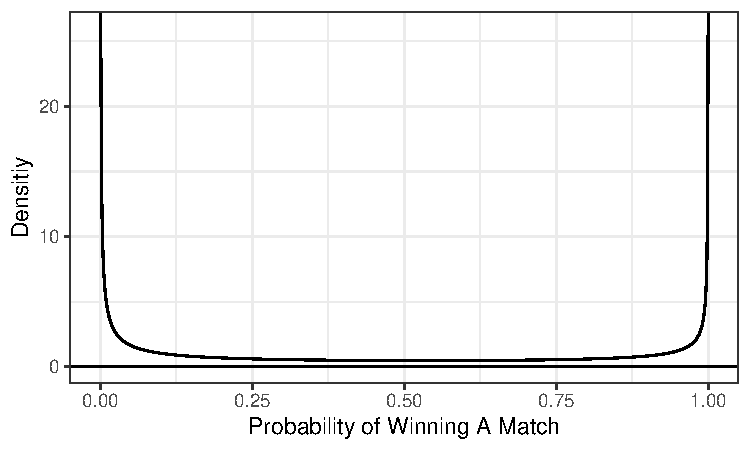
\includegraphics[keepaspectratio]{Lab10WriteUp_files/figure-pdf/fig-p1-1.pdf}}

}

\end{figure}%

\normalsize

\scriptsize

\begin{Shaded}
\begin{Highlighting}[numbers=left,,]
\NormalTok{plots[[}\DecValTok{2}\NormalTok{]] }
\end{Highlighting}
\end{Shaded}

\begin{figure}[H]

\caption{\label{fig-p2}Probability of winning a match for Luke
Humphries}

\centering{

\pandocbounded{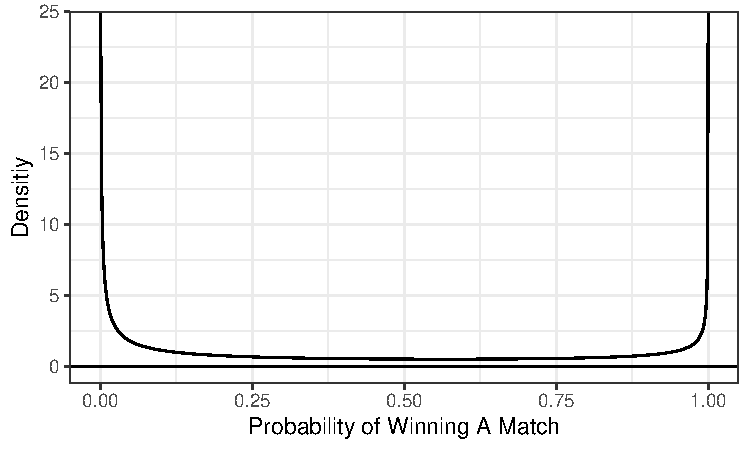
\includegraphics[keepaspectratio]{Lab10WriteUp_files/figure-pdf/fig-p2-1.pdf}}

}

\end{figure}%

\normalsize

\scriptsize

\begin{Shaded}
\begin{Highlighting}[numbers=left,,]
\NormalTok{plots[[}\DecValTok{3}\NormalTok{]] }
\end{Highlighting}
\end{Shaded}

\begin{figure}[H]

\caption{\label{fig-p3}Probability of winning a match for Michael van
Gerwen}

\centering{

\pandocbounded{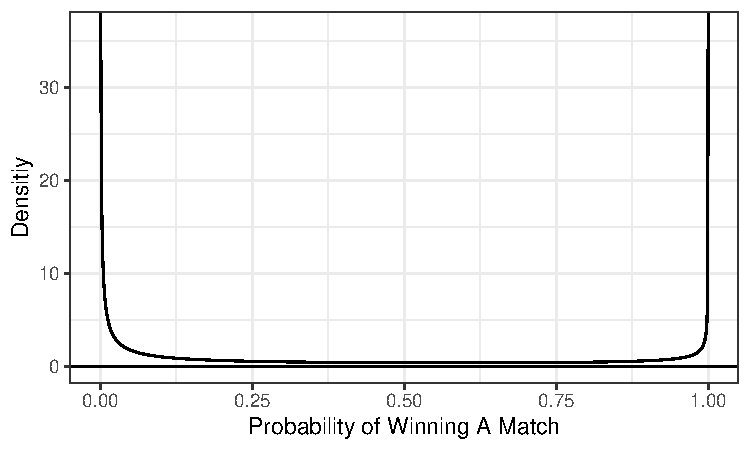
\includegraphics[keepaspectratio]{Lab10WriteUp_files/figure-pdf/fig-p3-1.pdf}}

}

\end{figure}%

\normalsize

\scriptsize

\begin{Shaded}
\begin{Highlighting}[numbers=left,,]
\NormalTok{plots[[}\DecValTok{4}\NormalTok{]] }
\end{Highlighting}
\end{Shaded}

\begin{figure}[H]

\caption{\label{fig-p4}Probability of winning a match for Michael Smith}

\centering{

\pandocbounded{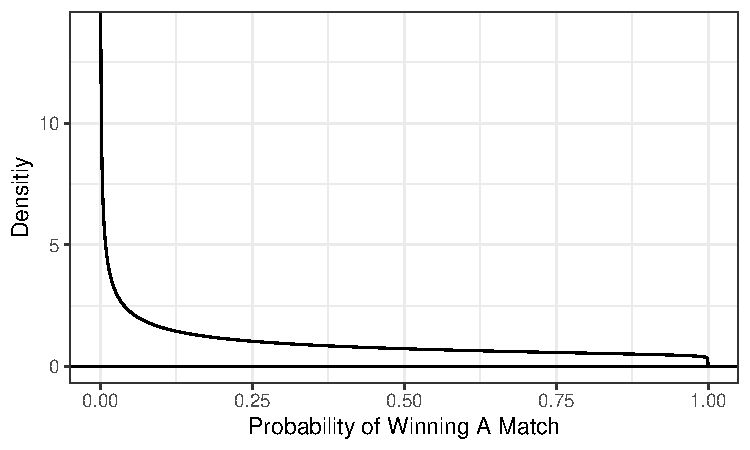
\includegraphics[keepaspectratio]{Lab10WriteUp_files/figure-pdf/fig-p4-1.pdf}}

}

\end{figure}%

\normalsize

\scriptsize

\begin{Shaded}
\begin{Highlighting}[numbers=left,,]
\NormalTok{plots[[}\DecValTok{5}\NormalTok{]] }
\end{Highlighting}
\end{Shaded}

\begin{figure}[H]

\caption{\label{fig-p5}Probability of winning a match for Nathan
Aspinall}

\centering{

\pandocbounded{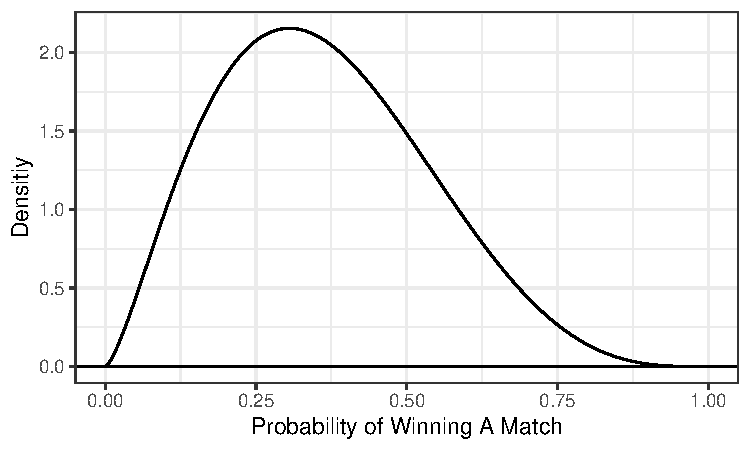
\includegraphics[keepaspectratio]{Lab10WriteUp_files/figure-pdf/fig-p5-1.pdf}}

}

\end{figure}%

\normalsize

\scriptsize

\begin{Shaded}
\begin{Highlighting}[numbers=left,,]
\NormalTok{plots[[}\DecValTok{6}\NormalTok{]] }
\end{Highlighting}
\end{Shaded}

\begin{figure}[H]

\caption{\label{fig-p6}Probability of winning a match for Rob Cross}

\centering{

\pandocbounded{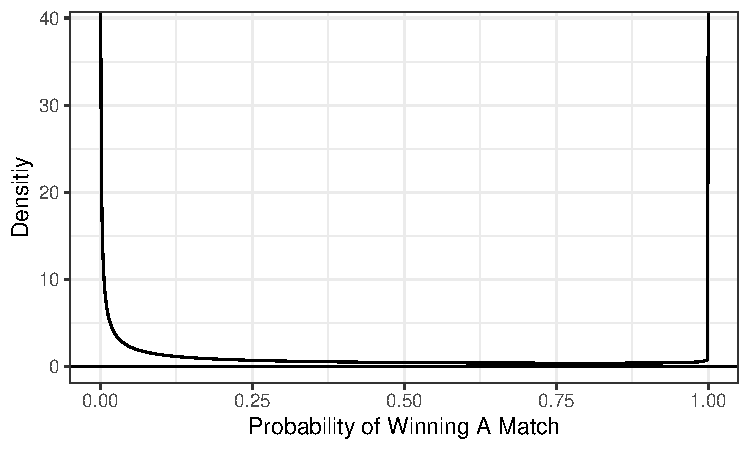
\includegraphics[keepaspectratio]{Lab10WriteUp_files/figure-pdf/fig-p6-1.pdf}}

}

\end{figure}%

\normalsize

\scriptsize

\begin{Shaded}
\begin{Highlighting}[numbers=left,,]
\NormalTok{plots[[}\DecValTok{7}\NormalTok{]] }
\end{Highlighting}
\end{Shaded}

\begin{figure}[H]

\caption{\label{fig-p7}Probability of winning a match for Gerwyn Price}

\centering{

\pandocbounded{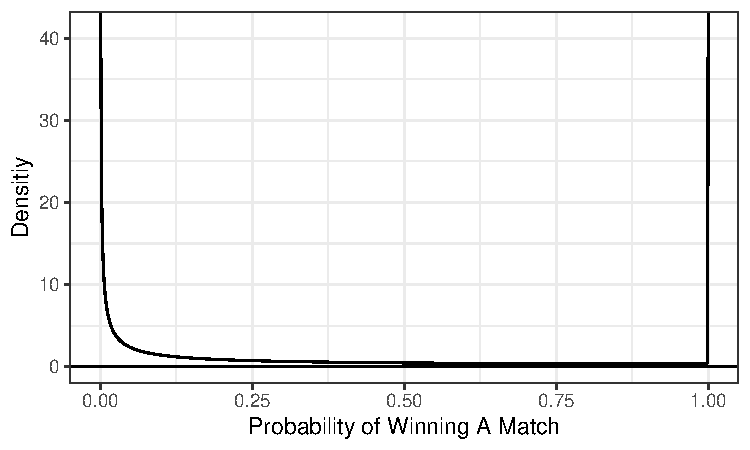
\includegraphics[keepaspectratio]{Lab10WriteUp_files/figure-pdf/fig-p7-1.pdf}}

}

\end{figure}%

\normalsize

\scriptsize

\begin{Shaded}
\begin{Highlighting}[numbers=left,,]
\NormalTok{plots[[}\DecValTok{8}\NormalTok{]] }
\end{Highlighting}
\end{Shaded}

\begin{figure}[H]

\caption{\label{fig-p8}Probability of winning a match for Peter Wright}

\centering{

\pandocbounded{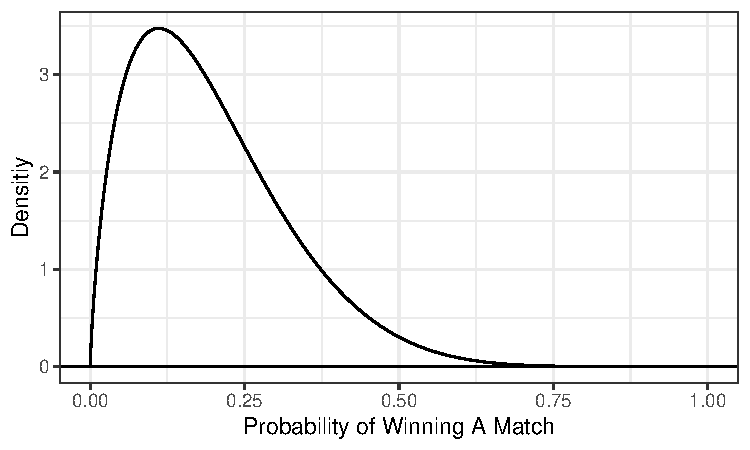
\includegraphics[keepaspectratio]{Lab10WriteUp_files/figure-pdf/fig-p8-1.pdf}}

}

\end{figure}%

\normalsize

The beta distribution is a distribution of the probability of winning
each leg for each player. Player 8, Peter Wright, have a right-skewed
and more narrow beta distribution. This means that his probability of
winning each leg is much less variable and consistently low. The
probability of Peter Wright having a 50\% chance of winning 1 leg is
very low. The probability of winning each leg for Player 5, Nathan
Aspinall, has a slightly right-skewed Beta distribution.

For the rest of the players, the Beta distribution plots for has a
U-shape (high density near 0 and 1). This means that the probability of
winning each leg is highly variable, either really high or really low.
Notably, Luke Littler has \(\theta=10.80\) and Luke Humphries has
\(\theta=6.39\), meaning their legs won alternate and almost don't
cluster--they often play very competitive, close matches.

\subsection{Executive Summary}\label{executive-summary}

Summarize the work you've done here to provide a brief (200-300 word)
data-driven summary of the 2024 Premier League season using your work in
Lab 10. Your summary should be professional, clear, and all claims
should be corroborated with statistical support.

\textbf{Solution}

The 2024 Premier League featured 8 best dart players, who competed in
best-of-11-leg matches. Each player starts out with 501 points, and as
they throw, points are subtracted, so the player who throws first in a
leg has the mathematical ``head start'' to reach a finish before their
opponent takes another turn.

Luke Littler and Luke Humphries are the most dominant players. Excluding
playoffs, they won 55\% and 56\% of total legs played respectively. The
estimates of their probability of winning each leg, as modelled by
Altham's Multiplicative Binomial Distributions, are 0.46 and 0.47,
respectively (adjusted for uncertainty in players' skills). Peter Wright
was the worst player of the season, winning only 37\% of legs played and
finishing with a leg spread of -43. Based on his Altham's Multiplicative
Beta Binomial Distribution, his probability of winning each leg is
consistently low.

Over half (53\%) of the matches have a score of 6-5 or 6-4, meaning most
of them are close and competitive and players only win in the
second-to-last or last leg. This is expected since the league is
composed of world-class players.

Looking at the Altham's Multiplicative Beta Binomial Distributions,
except for Peter Wright and Nathan Aspinall, the probability of winning
each leg for each player is highly variable. Thus, some nights they are
very likely to win the match, while some nights it's very competitive.




\end{document}
